\documentclass[../main/main.tex]{subfiles}


\begin{document}

\section{October  6th, 2020}
\subsection{Explicit Scheme for Hyperbolic Equation}
Applying the explicit scheme method, we have: \[
    \frac{U_{j}^{n+1}-U_j^n}{\Delta t} + a \frac{U_{j+1}^n - U_j^n}{\Delta x } = 0
.\] If we set $\nu = \frac{a \Delta t}{\Delta x}$, we have: \[
U^{n+1}_j = U^n_j - \nu (U_{j+1}^n - U_j^n) = (1+\nu) U_j^n - \nu U_{j+1}^n
.\] 
\begin{definition}[\vocab{CFL Condition}]
   For a convergent scheme, the domain of dependence of the PDE must lie within the domain of dependence of the numerical scheme. 
\end{definition}
\begin{example}
    The scheme above cannot converge for $a>0$. This is because if $a>0$, $U_j^{n+1}$ depends on  $U_j^n$,  $U_{j+1}^n$, $U_{j+1}^{n-1}$, $U_{j+2}^{n-1}$, etc. However, the characteristic line $x = at + x_0$ does not lie in this domain, thus the scheme does not hold.
\end{example}
\begin{example}
   If we instead use a backward difference: \[ 
       U^{n+1}_j = U^n_j - \nu (U_{j}^n - U_{j-1}^n) = (1+\nu) U_j^n - \nu U_{j}^n
   .\]  Then the characteristic line falls within the domain.
\end{example}
\begin{example}
    For $a < 0$, we must have $a \frac{\Delta t}{\Delta x}\le 1$, in order to have the characteristic line to lie within the domain.
\end{example}
If we attempt to use central difference, we can eliminate the sign condition by using a symmetric scheme in space: \[
    \frac{U_j^{n+1}-U_j^n}{\Delta t} + a \frac{U_{j+1}^n - U_{j-1}^n}{2\Delta x} = 0
.\] Note that for this scheme, CFL condition holds for $|a \frac{\Delta t}{\Delta x}| \le  1$. However, if we look at this from stability analysis, we have: \[
\frac{\lambda-1}{\Delta t} \lambda^n e^{ik(j\Delta x)} + \frac{a}{2\Delta x} \lambda^n e^{ik(j\Delta x)}\left( e^{ik\Delta x} - e ^{-ik\Delta x} \right) =0
.\] \[
 \implies \lambda = 1 - a \frac{\Delta t}{\Delta x} i \sin k\Delta x 
.\]which is complex. Thus we have: \[
|\lambda| = \sqrt{1+a^2\left( \frac{\Delta t}{\Delta x} \right)^2 \sin^2 k\Delta x }> 1 
.\] meaning it does not converge. Thus we cannot central difference for an explicit scheme for hyperbolic equation. Instead, we have to use forward or backwards depending on the value of $a$: \[
U^{n+1}_j = \begin{cases}
    U_j^n - \nu (U_{j+1}^n - U_j^n) & a < 0 \\
    U_j^n - \nu(U_j^n - U_{j-1}^n) & a > 0
\end{cases}
.\] which is called the \vocab{upwind scheme}.
\begin{example}
    In laymen terms, if the wave is going forward ($a>0$) we use backward difference, if the wave is going backward we use forward difference. 
\end{example}
Analyzing the stability, for $a>0$, (backward difference) we have:
\begin{align*} 
    \lambda &= 1 - \nu(1-e^{-ik\Delta x})\\
            &= 1-\nu(1-(\cos k\Delta x - i \sin k \Delta x)) \\
            &= 1-\nu(1-\cos k \Delta x) + i \nu \sin k \Delta x \\
    \implies |\lambda|^2 &= (1-\nu(1-\cos k\Delta x))^2 + \nu^2 \sin^2 k \Delta x \\
                         &= 1 - 2\nu (1-\nu) (1-\cos k\Delta x) \\
                         &= 1-4\nu(1-\nu) \sin^2 \left( \frac{1}{2}k \Delta x \right) < 1 \quad\text{ if }\nu<1
.\end{align*}
This matches the CFL condition. 
\begin{remark}
    Since this only uses first order derivatives, this scheme is only first order in time and space.
\end{remark}
Previously to get second order accuracy, we used central difference. However, as we showed above, this is not a stable scheme. To achieve this accuracy, we will use quadratic interpolation.
\section{Lax-Wendroff Scheme}
Suppose we want to find the value at $P$ in Figure \ref{10-6-lws}.
\begin{figure}[htpb]
    \centering
    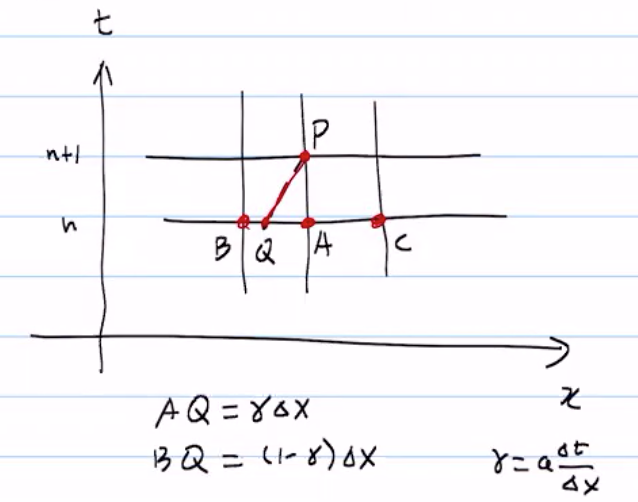
\includegraphics[width=0.5\textwidth]{10-6-lws}
    \caption{}
    \label{10-6-lws}
\end{figure}
Using the characteristic line, we have that $U(P) = U(Q)$, and as such, we want to find the value at $Q$. To do this, we can try linear interpolation with points $B = U^n_{j-1}, $ $A=U^n_j$, and $C=U_{j+1}^n$ that lie on the lattice:
\begin{align*}
    U(Q) &= \nu U(B) + (1-\nu)U(A) \\
    \implies U_j^{n+1} &= \nu U_{j-1}^n + (1-\nu)U^n_j
.\end{align*} which is exactly the upwind scheme. If we try quadratic interpolation, we would have:
In other words 
\begin{align*} 
    P(x) = U_{j-1} \frac{(x-\Delta x)}{(0 - \Delta x)}\cdot \frac{(x-2\Delta x)}{(0-2\Delta x)} + U_j \frac{(x-0)}{(\Delta x - 0)}\cdot  \frac{(x-2\Delta x)}{(\Delta x - 2 \Delta x)} + U_{j+1} \frac{(x-0)}{(2\Delta x-0)} \cdot  \frac{(x-\Delta x)}{(2\Delta x - \Delta x)}
.\end{align*} Plugging in $Q = (1-\nu) \Delta x$, we have:
\begin{align*}
    P(Q) &= \frac{\nu}{2}(1+\nu) U_{j-1} + (1-\nu)(1+\nu) U_j - \frac{1}{2}\nu(1-\nu) U_{j+1}\\
    \implies U^{n+1}_j &= U^n_j + \frac{\nu}{2}(U^n_{j-1}U^n_{j+1})+\frac{\nu^2}{2}\left( U_{j-1}^n - 2U^n_j + U_{j+1}^n \right) 
.\end{align*}
Remember we need the characteristic line to lie within the scheme to satisfy the CFL condition, meaning we need  $|\nu| \le  1$. This scheme is called the \vocab{Lax-Wendroff method}.
\begin{remark}
   Note that this scheme is similar to the central difference but with a higher order correction term. 
\end{remark}
\begin{remark}
    The above scheme is second order in space. This can be verified by calculating the truncation error.
\end{remark}
Checking the stability analysis, we would have: 
\begin{align*}
    \lambda &= (1-2\nu^2\sin^2 \frac{k\Delta x}{2})^2 + \nu^2 \sin^2 k \Delta x \\
    |\lambda|^2&= (1-2\nu^2 \sin^2 \frac{k\Delta x}{2})^2 + \nu^2 \sin^2 k\Delta x \\
    &= 1-4\nu^2 \sin^2 \frac{k\Delta x}{2}+ 4 \nu^4 \sin^4 \frac{k\Delta x}{2}+4\nu^2 \sin^2 \frac{k\Delta x}{2} \cos^2 \frac{k\Delta x}{2} \\
    &= 1-4\nu^2(1-\nu^2)\sin^{4}\left(\frac{1}{2} k\Delta x\right) \le  1\quad \text{ if }\nu \le  1 \\
.\end{align*} This means the scheme is stable for $|\nu|\le  1$ (CFL condition). 

To summarize, the design of numerical methods for hyperbolic equations is very different that for parabolic equations, as the issues we have to consider are very different.
\end{document}


